\begin{blocksection}
\question Draw the environment diagram that results from running the code below.

\begin{questionmeta}
    It may be helpful to give students an overview on the rules of drawing environment diagrams, such as when to open new frames, how to format the frames, what parent frames are, when to draw pointers to objects, frame hierarchy, lambdas, and any tips/tricks you may think of!
\end{questionmeta}

\begin{lstlisting}
def dream1(f):
    def dream2(secret):
        mind = f(secret)
        kick = lambda x: mind()
        return kick(2)
    return dream2

inception = lambda secret: lambda: secret
real = dream1(inception)(42)
\end{lstlisting}

\pagebreak

\begin{solution}[2in]
Output: 42 \newline
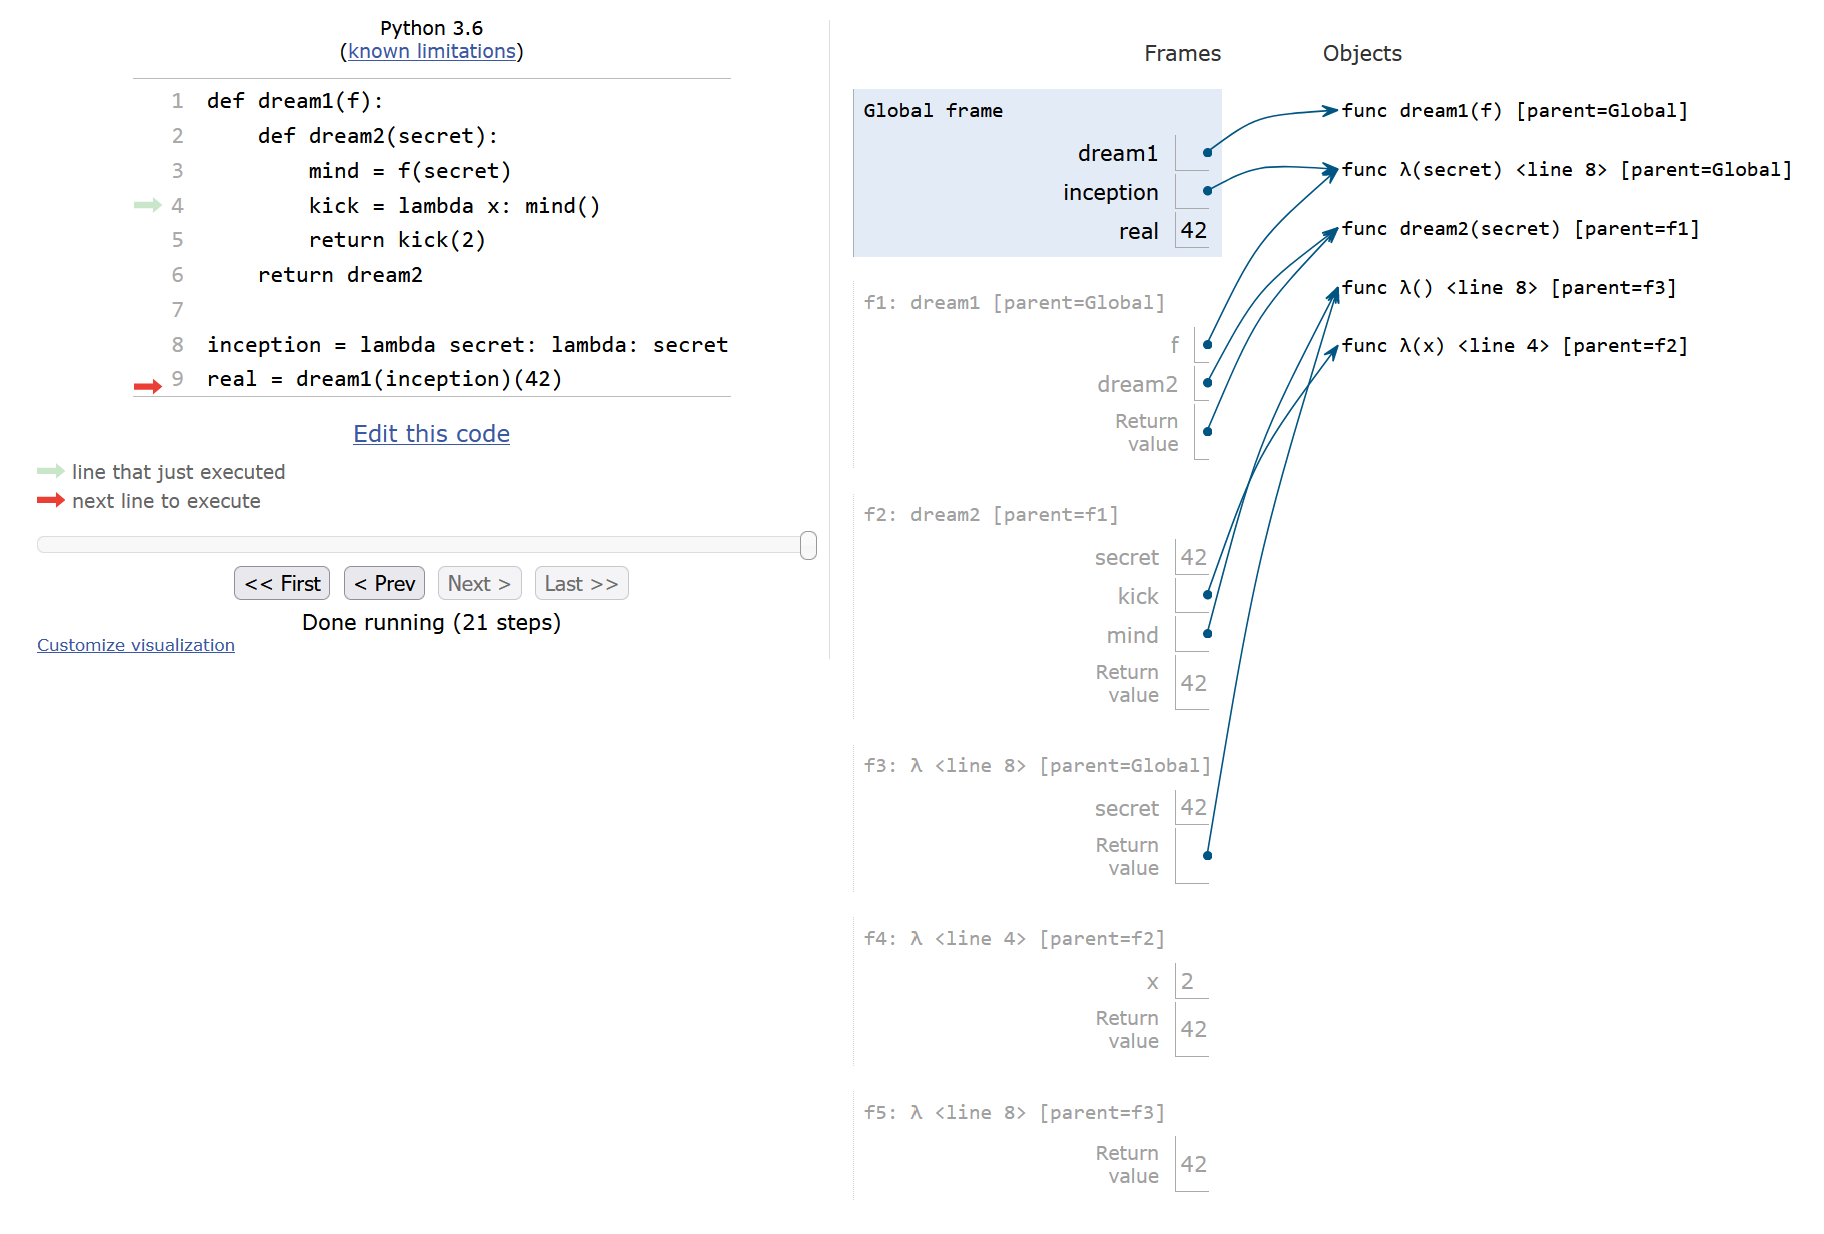
\includegraphics[scale=0.5]{newNewInception.png}
\newline
\url{https://imgur.com/a/ZKwZzdy}
\end{solution}
\end{blocksection}
